\documentclass[12pt]{beamer}
\usepackage{../Estilos/BeamerMAF}
\usetheme{Warsaw}
\usecolortheme{seahorse}
%\useoutertheme{default}
\setbeamercovered{invisible}
% or whatever (possibly just delete it)
\setbeamertemplate{section in toc}[sections numbered]
\setbeamertemplate{subsection in toc}[subsections numbered]
\setbeamertemplate{subsection in toc}{\leavevmode\leftskip=3.2em\rlap{\hskip-2em\inserttocsectionnumber.\inserttocsubsectionnumber}\inserttocsubsection\par}
\setbeamercolor{section in toc}{fg=blue}
\setbeamercolor{subsection in toc}{fg=blue}
\setbeamercolor{frametitle}{fg=blue}
\setbeamertemplate{caption}[numbered]

\setbeamertemplate{footline}
\beamertemplatenavigationsymbolsempty
\setbeamertemplate{headline}{}


\makeatletter
\setbeamercolor{section in foot}{bg=gray!30, fg=black!90!orange}
\setbeamercolor{subsection in foot}{bg=blue!30}
\setbeamercolor{date in foot}{bg=black}
\setbeamertemplate{footline}
{
  \leavevmode%
  \hbox{%
  \begin{beamercolorbox}[wd=.333333\paperwidth,ht=2.25ex,dp=1ex,center]{section in foot}%
    \usebeamerfont{section in foot} \insertsection
  \end{beamercolorbox}%
  \begin{beamercolorbox}[wd=.333333\paperwidth,ht=2.25ex,dp=1ex,center]{subsection in foot}%
    \usebeamerfont{subsection in foot}  \insertsubsection
  \end{beamercolorbox}%
  \begin{beamercolorbox}[wd=.333333\paperwidth,ht=2.25ex,dp=1ex,right]{date in head/foot}%
    \usebeamerfont{date in head/foot} \insertshortdate{} \hspace*{2em}
    \insertframenumber{} / \inserttotalframenumber \hspace*{2ex} 
  \end{beamercolorbox}}%
  \vskip0pt%
}
\makeatother

\makeatletter
\patchcmd{\beamer@sectionintoc}{\vskip1.5em}{\vskip0.8em}{}{}
\makeatother

\newlength{\depthofsumsign}
\setlength{\depthofsumsign}{\depthof{$\sum$}}
\newcommand{\nsum}[1][1.4]{% only for \displaystyle
    \mathop{%
        \raisebox
            {-#1\depthofsumsign+1\depthofsumsign}
            {\scalebox
                {#1}
                {$\displaystyle\sum$}%
            }
    }
}
\def\scaleint#1{\vcenter{\hbox{\scaleto[3ex]{\displaystyle\int}{#1}}}}
\def\scaleoint#1{\vcenter{\hbox{\scaleto[3ex]{\displaystyle\oint}{#1}}}}
\def\bs{\mkern-12mu}

\makeatletter
% \setbeamercolor{section in foot}{bg=gray!30, fg=black!90!orange}
% \setbeamercolor{subsection in foot}{bg=blue!30!yellow, fg=red}
% \setbeamercolor{date in foot}{bg=black, fg=white}
\setbeamertemplate{footline}
{
  \leavevmode%
  \hbox{%
  \begin{beamercolorbox}[wd=.333333\paperwidth,ht=2.25ex,dp=1ex,center]{section in foot}%
    \usebeamerfont{section in foot} \insertsection
  \end{beamercolorbox}%
  \begin{beamercolorbox}[wd=.333333\paperwidth,ht=2.25ex,dp=1ex,center]{subsection in foot}%
    \usebeamerfont{subsection in foot}  \insertsubsection
  \end{beamercolorbox}%
  \begin{beamercolorbox}[wd=.333333\paperwidth,ht=2.25ex,dp=1ex,right]{date in head/foot}%
    \usebeamerfont{date in head/foot} \insertshortdate{} \hspace*{2em}
    \insertframenumber{} / \inserttotalframenumber \hspace*{2ex} 
  \end{beamercolorbox}}%
  \vskip0pt%
}
\makeatother
\date{20 de septiembre de 2021}
\title{Objetivos del Tema 1}
\subtitle{La física y la geometría}
\begin{document}
\maketitle
\fontsize{14}{14}\selectfont
\spanishdecimal{.}
\section*{Contenido}
\frame[allowframebreaks]{\tableofcontents[currentsection, hideallsubsections]}
\section{Introducción}
\frame[allowframebreaks]{\tableofcontents[currentsection, hideothersubsections]}
\subsection{Sistemas conocidos}
\begin{frame}
\frametitle{Introducción}
Estamos familiarizados con el uso de distintos sistemas coordenados para describir problemas físicos.
\\
\bigskip
\pause
Hemos usado coordenadas cartesianas, cilíndricas y esféricas para problemas con esas simetrías.
\end{frame}
\begin{frame}
\frametitle{Otros sistemas}
Veremos que existen otros sistemas coordenados que poco a poco durante la carrera, nos encontraremos con ellos para problemas en particular.
\\
\bigskip
\pause
El Tema 1 nos brindará una estrategia de trabajo con ellos.
\end{frame}
\section{Ejemplos}
\frame{\tableofcontents[currentsection, hideothersubsections]}
\subsection{Dos ejemplos}
\begin{frame}
\frametitle{Primer ejemplo}
Consideremos el vector campo eléctrico $(\va{E})$ creado por una carga puntual $q$ localizada en el origen de un sistema cartesiano. \pause Usando los vectores de la base canónica en $\mathbb{R}^{3}$, el campo es:
\pause
\begin{align*}
\va{E} = \dfrac{q}{4 \pi \varepsilon_{0}} \, \dfrac{x \, \vu{e}_{x} + y \, \vu{e}_{y} + z \, \vu{e}_{z}}{\left( x^{2} + y^{2} + z^{2} \right)^{3/2}}
\end{align*}
\end{frame}
\begin{frame}
\frametitle{Primer ejemplo}
En coordenadas esféricas $(r, \theta, \phi)$, en donde se aprovecha completamente la simetría del problema para este campo, se simplifica la expresión anterior, \pause así el campo eléctrico resulta ser:
\begin{align*}
\va{\vb{E}} = \dfrac{q}{4 \pi \varepsilon_{0}} \, \dfrac{\vu{e}_{r}}{r^{2}}
\end{align*}
\end{frame}
\begin{frame}
\frametitle{¿Cómo cambiamos de un sistema a otro?}
Será necesario utilizar conceptos como reglas de transformación, factores de escala, vectores unitarios, así como representar en el nuevo sistema coordenado, el conjunto de operadores diferenciales que ya conocemos: gradiente, divergencia y rotacional.
\end{frame}
\begin{frame}
\frametitle{Segundo ejemplo}
Ahora consideramos un problema con ondas estacionarias en un sistema bidimensional con simetría circular: una membrana circular delgada y perfectamente flexible, por ejemplo: una membrana de tambor circular idealizada de radio $r$.
\pause
\begin{figure}[H]
  \centering
  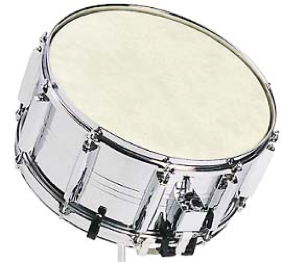
\includegraphics[scale=0.75]{Imagenes/Tambor.png}
\end{figure}
\end{frame}
\begin{frame}
\frametitle{Segundo ejemplo}
La ecuación de onda en coordenadas bidimensionales cilíndricas $(x , y \rightarrow r, \varphi)$ para la amplitud de desplazamiento, $\psi (r, \varphi, t)$ viene dada por:
\pause
\begin{align*}
\laplacian \psi (r, \varphi, t) - \dfrac{1}{v^{2}} \pdv[2]{\psi (r, \varphi, t)}{t} = 0
\end{align*}
\end{frame}
\begin{frame}
\frametitle{Elegir el sistema coordenado}
Para la elección del sistema coordenado debemos de considerar aquel en donde la simetría del problema nos simplique el trabajo.
\\
\bigskip
\pause
En este caso, corresponde elegir el sistema coordenado cilíndrico.
\end{frame}
\begin{frame}
\frametitle{Geometría del sistema cilíndrico}
\begin{figure}[H]
  \centering
  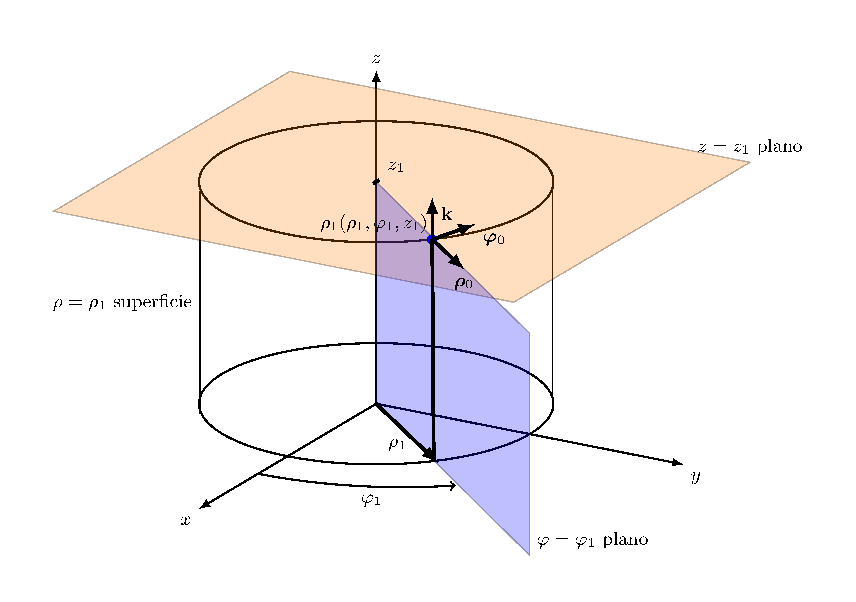
\includegraphics[scale=0.7]{Imagenes/Coordenadas_Cilindricas_01.eps}
\end{figure}
\end{frame}
\begin{frame}
\frametitle{Reexpresar la ecuación de onda}
Una vez elegido el sistema coordenado, debemos de realizar lo necesario para reexpresar la ecuación diferencial del problema en el sistema.
\\
\bigskip
\pause
Habrá que \enquote{adaptar} el operador Laplaciano en este sistema.
\end{frame}
\begin{frame}
\frametitle{Solución a la ED obtenida}
Una vez que se realiza la reexpresión de la ED, el siguiente paso es resolverla.
\\
\bigskip
\pause
Para ello, ocuparemos lo que se revisará en el \emph{\textcolor{blue}{Tema 2 - Primeras técnicas de solución}}.
\end{frame}
\begin{frame}
\frametitle{Solución al problema}
Cuando veamos el tema de \emph{función de Bessel}, tomaremos de nuevo este ejercicio.
\\
\bigskip
\pause
La solución obtenida la podemos ocupar con otras herramientas computacionales para \emph{simular} el comportamiento de la membrana circular.
\end{frame}
\begin{frame}
\frametitle{Simulación computacional}
\begin{figure}[h!]
    \centering
    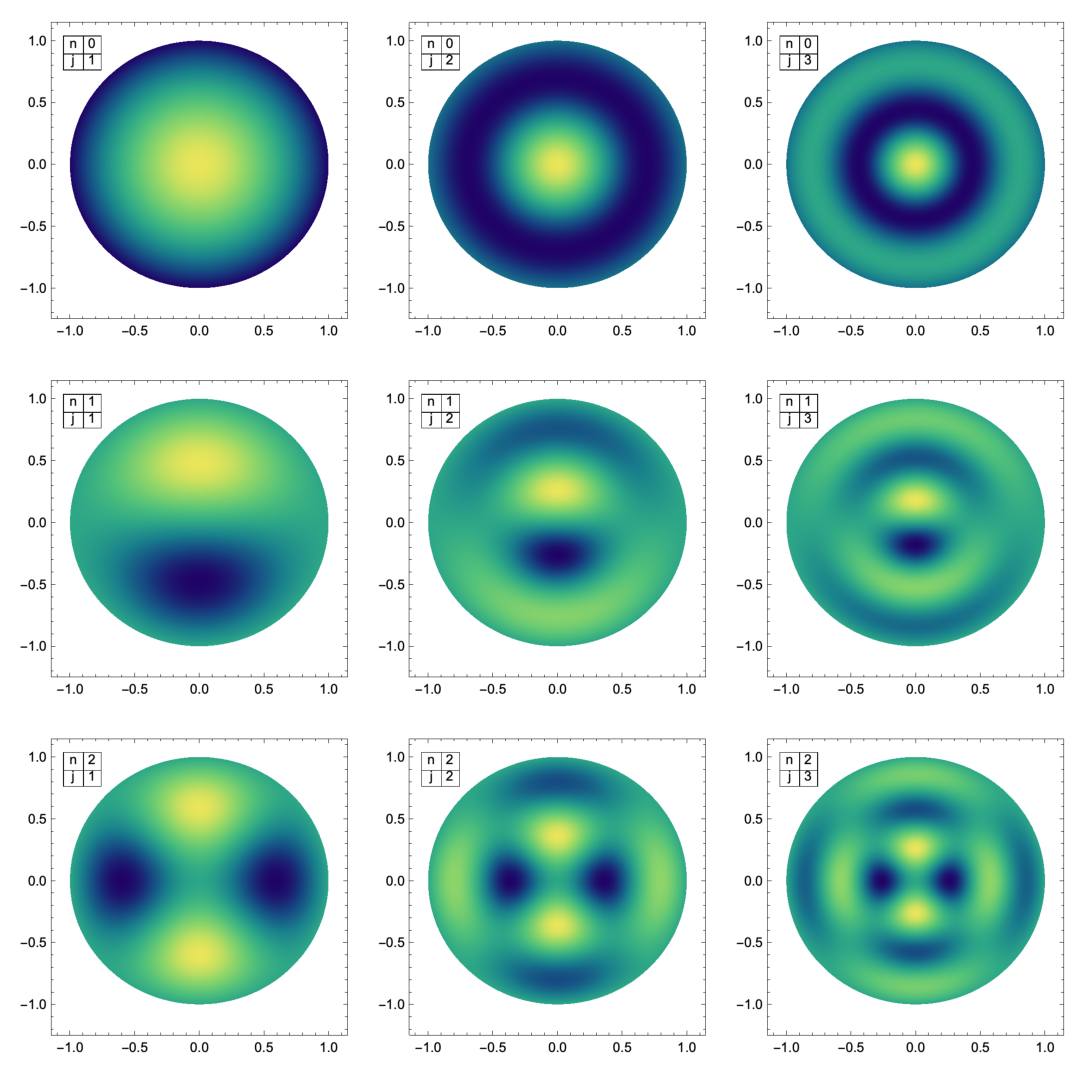
\includegraphics[scale=0.32]{Imagenes/Modos_Vibracion_Membrana_Circular_01.eps}
\end{figure}
\end{frame}
\begin{frame}
\frametitle{¿Y si tenemos un toroide?}
\begin{figure}
    \centering
    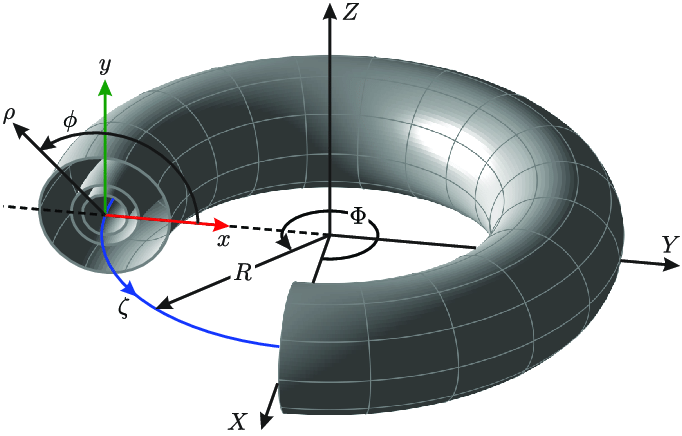
\includegraphics[scale=0.4]{Imagenes/Geometria_Toro.png}
\end{figure}
\end{frame}
\begin{frame}
\frametitle{Sistemas coordenados}
\setbeamercolor{item projected}{bg=blue!70!black,fg=yellow}
\setbeamertemplate{enumerate items}[circle]
\begin{enumerate}[<+->]
\item Esféricas polares.
\item Cilíndricas polares.
\item Cilíndricas parabólicas.
\item Parabólicas.
\item Cilíndricas elípticas.
\item Esferoidales prolatas.
\item Esferoidales oblatas.
\seti
\end{enumerate}
\end{frame}
\begin{frame}
\frametitle{Sistemas coordenados}
\setbeamercolor{item projected}{bg=blue!70!black,fg=yellow}
\setbeamertemplate{enumerate items}[circle]
\begin{enumerate}[<+->]
\conti
\item Elipsoidal.
\item Toroidal.
\item Cilíndricas bipolares.
\item Biesféricas.
\item Cónicas.
\item Cardioide.
\end{enumerate}
\end{frame}
\begin{frame}
\frametitle{La ecuación de Helmholtz}
La ecuación de Helmholtz se encuentra muy a menudo en la física:
\pause
\begin{align*}
\laplacian{\psi} + k \, \psi = 0
\end{align*}
\pause
Con lo que veremos en el Tema 1 y al inicio del Tema 2, encontramos que la ecuación es \emph{separable} en 11 de los sistemas coordenados mencionados previamente.
\end{frame}

\section{Objetivos}
\frame{\tableofcontents[currentsection, hideothersubsections]}
\subsection{Tema 1}

\begin{frame}
\frametitle{Objetivos}
Al concluir el Tema 1, el alumno:
\setbeamercolor{item projected}{bg=blue!70!black,fg=yellow}
\setbeamertemplate{enumerate items}[circle]
\begin{enumerate}[<+->]
\item Describirá las superficies coordenadas a partir de las reglas de transformación entre el sistema cartesiano y otro sistema de estudio.
\item Determinará los factores de escala del nuevo sistema de estudio, así como los vectores base y la interpretación con los vectores cartesianos.
\seti
\end{enumerate}
\end{frame}
\begin{frame}
\frametitle{Objetivos}
\setbeamercolor{item projected}{bg=blue!70!black,fg=yellow}
\setbeamertemplate{enumerate items}[circle]
\begin{enumerate}[<+->]
\conti
\item Calculará los operadores diferenciales en el nuevo sistema de estudio.
\item Resolverá mediante las funciones Gamma y Beta ejercicios de la física.
\end{enumerate}
\end{frame}
\section{Trabajo asíncrono}
\frame{\tableofcontents[currentsection, hideothersubsections]}
\subsection{Presentaciones}
\begin{frame}
\frametitle{Trabajo a realizar}
Como se revisó en la presentación del curso de MAF, el trabajo asíncrono por parte del alumno, consistirá en leer los materiales del curso en la plataforma Moodle, siendo los siguientes:
\end{frame}
\begin{frame}
\frametitle{Materiales de trabajo}
\setbeamercolor{item projected}{bg=blue!70!black,fg=yellow}
\setbeamertemplate{enumerate items}[circle]
\begin{enumerate}[<+->]
\item 1 - Sistema de coordenadas curvilíneas ortogonales.
\item 2 - Diferenciales y operadores diferenciales.
\item 3 - Construcción de sistemas coordenados especiales.
\item 4 - Funciones Gamma y Beta.
\end{enumerate}
\end{frame}
\begin{frame}
\frametitle{Trabajo por semana}
Recomendación para la revisión de materiales de trabajo por semana:
\setbeamercolor{item projected}{bg=blue!70!black,fg=yellow}
\setbeamertemplate{enumerate items}[circle]
\begin{enumerate}[<+->]
\item Semana 1: Materiales de trabajo 1 y 2.
\item Semana 2: Materiales de trabajo 3 y 4.
\end{enumerate}
\end{frame}
\begin{frame}
\frametitle{Envío de ejercicios a cuenta}
\setbeamercolor{item projected}{bg=blue!70!black,fg=yellow}
\setbeamertemplate{enumerate items}[circle]
\begin{enumerate}[<+->]
\item Semana 1: Ejercicios Material de trabajo 1 (un ejercicio), Material de trabajo 2 (los primeros tres ejercicios). Se entregarán el 12 de marzo.
\item Semana 2: Ejercicios Materiales de trabajo 2 (cinco ejercicios) y Material 3 (dos ejercicios). Se entregarán el 19 de marzo.
\item Semana 3: Ejercicio Material de trabajo 4: 2 ejercicios. Se entregarán el 26 de marzo.
\end{enumerate}
\end{frame}
\begin{frame}
\frametitle{Materiales complementarios}
Tendrán disponibles materiales complementarios, que como mencionamos en la presentación del curso, les serán de utilidad ya que cuentan con un enfoque elevado, pero lo necesario para una consulta.
\\
\bigskip
Siendo también un atractivo para que extiendan la consulta en las referencias bibliográficas del curso.
\end{frame}

\section{Sesiones síncronas}
\frame{\tableofcontents[currentsection, hideothersubsections]}

\subsection{Programa de videoconferencias}

\begin{frame}
\frametitle{Sesiones síncronas}
Hemos programado sesiones los días miércoles y viernes en un horario de 3 a 4 pm.
\\
\bigskip
\pause
En estas sesiones se trabajarán algunos ejercicios para complementar los materiales de trabajo, y se dará espacio para dudas, comentarios, etc. tanto de las presentaciones como de los ejercicios a cuenta.
\end{frame}
\begin{frame}
\frametitle{Calendario de reuniones}
\setbeamercolor{item projected}{bg=blue!70!black,fg=yellow}
\setbeamertemplate{enumerate items}[circle]
\begin{enumerate}[<+->]
\item Viernes 5 de marzo.
\item Miércoles 10 de marzo.
\item Viernes 12 de marzo.
\item Miércoles 17 de marzo.
\item Viernes 19 de marzo. 
\end{enumerate}
\end{frame}
\end{document}